\section{Base\-CDI.h File Reference}
\label{BaseCDI_8h}\index{BaseCDI.h@{BaseCDI.h}}
{\tt \#include $<$map$>$}\par
{\tt \#include $<$string$>$}\par
{\tt \#include \char`\"{}Double\_\-2D.h\char`\"{}}\par


This graph shows which files directly or indirectly include this file:\begin{figure}[H]
\begin{center}
\leavevmode
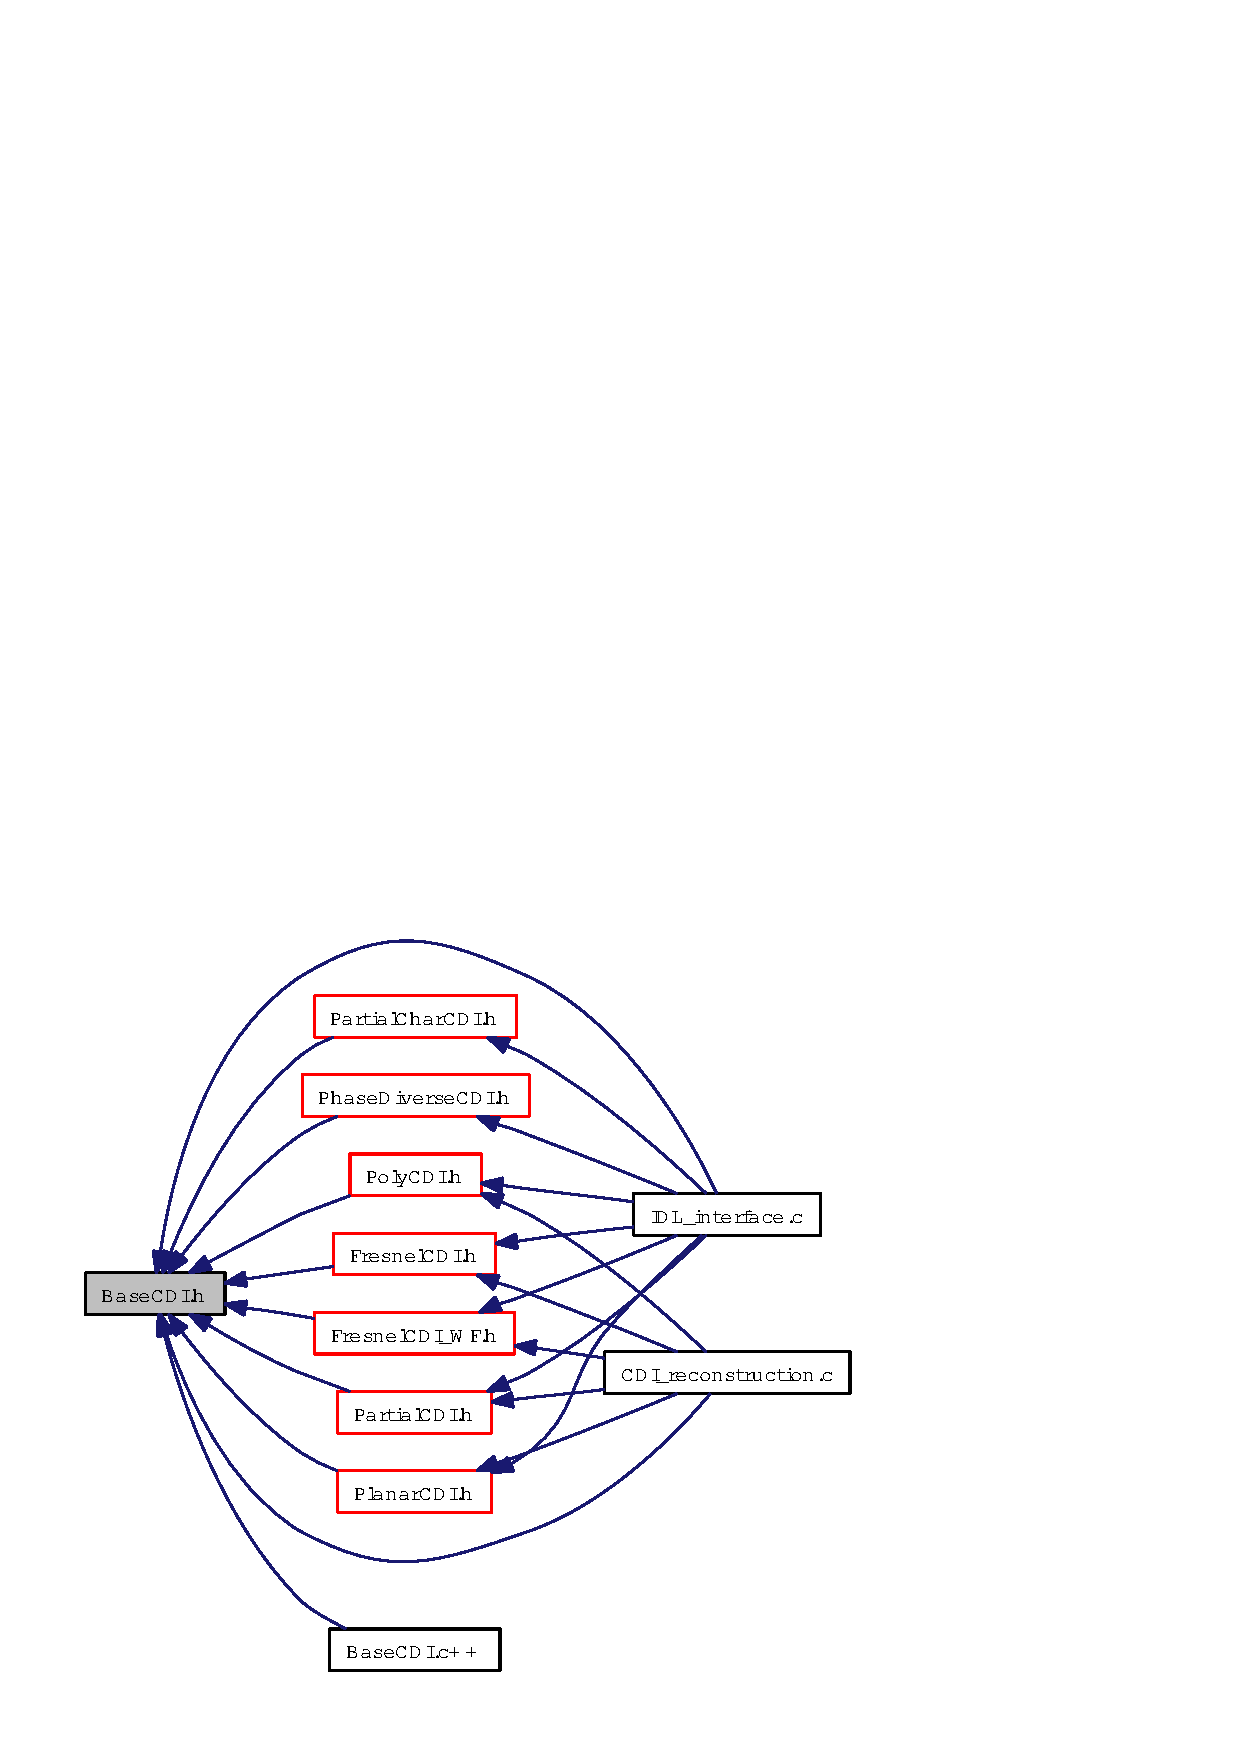
\includegraphics[width=206pt]{BaseCDI_8h__dep__incl}
\end{center}
\end{figure}
\subsection*{Data Structures}
\begin{CompactItemize}
\item 
class \bf{Base\-CDI}
\begin{CompactList}\small\item\em The class which performs planar CDI reconstruction. \item\end{CompactList}\end{CompactItemize}
\subsection*{Defines}
\begin{CompactItemize}
\item 
\#define \bf{NALGORITHMS}~9
\item 
\#define \bf{NTERMS}~5
\item 
\#define \bf{NVECTORS}~10
\end{CompactItemize}
\subsection*{Enumerations}
\begin{CompactItemize}
\item 
enum \{ \par
\textbf{PSF}, 
\textbf{PFS}, 
\textbf{PS}, 
\textbf{PF}, 
\par
\textbf{PI}
 \}
\item 
enum \{ \par
\textbf{ER}, 
\textbf{BIO}, 
\textbf{BOO}, 
\textbf{HIO}, 
\par
\textbf{DM}, 
\textbf{SF}, 
\textbf{ASR}, 
\textbf{HPR}, 
\par
\textbf{RAAR}, 
\textbf{CUSTOM}
 \}
\end{CompactItemize}


\subsection{Detailed Description}


Definition in file \bf{Base\-CDI.h}.

\subsection{Define Documentation}
\index{BaseCDI.h@{Base\-CDI.h}!NALGORITHMS@{NALGORITHMS}}
\index{NALGORITHMS@{NALGORITHMS}!BaseCDI.h@{Base\-CDI.h}}
\subsubsection{\setlength{\rightskip}{0pt plus 5cm}\#define NALGORITHMS~9}\label{BaseCDI_8h_da1f68143ff23653b8ca3e023e5048fb}


The number of reconstruction algorithms 

Definition at line 65 of file Base\-CDI.h.\index{BaseCDI.h@{Base\-CDI.h}!NTERMS@{NTERMS}}
\index{NTERMS@{NTERMS}!BaseCDI.h@{Base\-CDI.h}}
\subsubsection{\setlength{\rightskip}{0pt plus 5cm}\#define NTERMS~5}\label{BaseCDI_8h_aa111f26beb27a4bfca9e934283d81ac}


The number of unique combination projectors (i.e. terms) 

Definition at line 68 of file Base\-CDI.h.\index{BaseCDI.h@{Base\-CDI.h}!NVECTORS@{NVECTORS}}
\index{NVECTORS@{NVECTORS}!BaseCDI.h@{Base\-CDI.h}}
\subsubsection{\setlength{\rightskip}{0pt plus 5cm}\#define NVECTORS~10}\label{BaseCDI_8h_0ca34ffb02eaf6136977911eb748cb9e}


The number of unique combination of terms (ie. vectors) 

Definition at line 71 of file Base\-CDI.h.

\subsection{Enumeration Type Documentation}
\subsubsection{\setlength{\rightskip}{0pt plus 5cm}anonymous enum}\label{BaseCDI_8h_2e520baeab5e72a8cd84e00dce61684f}


The terms in the iteration equation 

Definition at line 74 of file Base\-CDI.h.\subsubsection{\setlength{\rightskip}{0pt plus 5cm}anonymous enum}\label{BaseCDI_8h_39b3af0f22dc1b8cb10e193d9fc491b4}


The different algorithms to choose from 

Definition at line 77 of file Base\-CDI.h.